\section{Introduction}
Sau khi đã hoàn thành \code{milestone-1} nhóm đã có được một ứng dụng cơ bản, có giao diện cho phép người dùng có thể chọn các file \code{svg} bất kỳ để hiển thị lên màn hình. Ứng dụng cũng đã được xây dựng để có thể hỗ trợ được các tính năng cơ bản cho việc tùy biến cũng như là nhu cầu của người dùng như là: \textit{Xoay, Phóng to, Thu nhỏ, Lật ngược}. 
Hiện tại, ứng dụng của nhóm đã có thể hỗ trợ các \code{tag} cơ bản của một file \code{svg} để có thể hiện thị các hình dạng cơ bảng như: \code{<rect>}, \code{<circle>}, \code{<ellipse>}, \code{<line>}, \code{<polyline>}, \code{<polygon>}, \code{<text>}. 

Tuy nhiên, nhu cầu của người dùng không chỉ dừng lại ở đó, các file \code{svg} được yêu cầu phải có thể chứa các hình ảnh phức tạp, có đường cong, đường uốn lượng, đường xiên ngang từ đó mà tạo nên tính sáng tạo và đa dạng của bức tranh hơn. Do đó nhóm đã thêm các tag để thực hiện được nhu cầu đó chính là: \code{<path>}. Việc thêm \code{<path>} nó cũng không phải là một thách thức quá lớn cho nhóm vì ngay từ ban đầu, nhóm đã thống nhất xây dựng theo các \code{design pattern} nào đó, thống nhất với về cách code, cũng như là tổ chức quản lý, do đó việc bảo trì và thêm tính năng đã được đơn giản hóa đi rất nhiều.

\section{GitHub Repository Link}
Nhằm phục vụ cho việc quản lý dự án, cũng như là công khai các mã nguồn có trong dự án thì nhóm cũng đã đẩy toàn bộ dự án lên trên \href{https://github.com/}{GitHub}:

\textbf{Link: } \href{https://github.com/khang1108/prototype-design-pattern}{See more}

\section{GitHub Commit List}
Để cung cấp một cái nhìn minh bạch và toàn diện về quá trình phát triển của dự án, dưới đây là toàn bộ lịch sử commit được trích xuất từ repository. Danh sách này được trình bày theo định dạng rút gọn, thể hiện các thay đổi, gộp nhánh và các cột mốc quan trọng từ khi bắt đầu cho đến khi hoàn thiện dự án.

% Sử dụng lstlisting để hiển thị code một cách ổn định và an toàn
\begin{lstlisting}[
    language=bash, 
    basicstyle=\ttfamily\scriptsize, % Font chữ TINY (rất nhỏ) để chứa được toàn bộ log
    breaklines=true,         % Tự động xuống dòng khi cần
    frame=single,            % Thêm khung bao quanh
    caption={Lịch sử commit đầy đủ của dự án NaTruKi},
    label=lst:gitlog_full
]
e72f2ea Nguyen Phuc Khang 2025-12-16
    merge to main
3bd57d2 Nguyen Phuc Khang 2025-12-16
    something fix
988844c pumpomeo 2025-12-16
    fix: scale function
4029ff6 pumpomeo 2025-12-16
    copy of B#2
5e7f9c5 nh996 2025-12-10
    FINAL (word alignment+color+rotation)
8360949 nh996 2025-12-08
    rotation on flipped image fix
c013f31 nh996 2025-11-22
    final
994a033 nh996 2025-11-21
    Add SVGPath element to "finish app"
e025c89 Nguyen Phuc Khang 2025-11-20
    merge files
bf974f5 Nguyen Phuc Khang 2025-11-20
    Merge branch 'main' of https://github.com/khang1108/natrukiSVG
9b68759 Nguyen Phuc Khang 2025-11-20
    add explaination for functions and add SVGPath
d73a87a Nguyen Phuc Khang 2025-11-19
    Update README.md (#6)
7b0cb8d Nguyen Phuc Khang 2025-11-19
    add some new features
cc31aad Nguyen Phuc Khang 2025-11-19
    finish application
71746d6 Nguyen Phuc Khang 2025-11-16
    Remove build artifacts and IDE files from repository
60527b6 Nguyen Phuc Khang 2025-11-16
    fix qt
8761aa0 Nguyen Phuc Khang 2025-11-16
    Merge remote-tracking branch 'origin/classdefining'
95451bc cpgod36 2025-11-15
    sua loi noi bo
0fa78f4 Nguyen Phuc Khang 2025-11-15
    fix main cmake
ca6b2c6 cpgod36 2025-11-12
    sua nut size
b143c1a cpgod36 2025-11-12
    hehe
c81019d cpgod36 2025-11-12
    latest
26235ae nh996 2025-11-11
    .
f8defdc nh996 2025-11-11
    Merge branch 'Parser+SceneGraph' of https://github.com/khang1108/natrukiSVG into Parser+SceneGraph
e2d8172 nh996 2025-11-11
    svgfactory adjustment
f4af068 cpgod36 2025-11-11
    moi nhat
2a7db1e nh996 2025-11-10
    Delete .vscode directory
86a297d nh996 2025-11-10
    Delete build directory
138dbf0 nh996 2025-11-10
    bug fix#1
bf6168e nh996 2025-11-10
    roleB
6f85fc5 cpgod36 2025-11-06
    add some actions on mainwindow
c393c1d cpgod36 2025-11-06
    resources/premium added
7f29609 cpgod36 2025-11-06
    da doi svg thanh png
3490f48 cpgod36 2025-11-06
    folder resources/about added
b35b95d cpgod36 2025-11-06
    upload resources
9211e62 cpgod36 2025-11-06
    include folder completed
86c759d cpgod36 2025-11-05
    Merge remote-tracking branch 'origin/main' into classdefining
da0ab28 cpgod36 2025-11-05
    Role A: folder /include/svg completed
497ded4 Nguyen Phuc Khang 2025-11-05
    Fix README.md
ed68102 Nguyen Phuc Khang 2025-11-05
    update CMakeLists
b84fef6 cpgod36 2025-11-05
    define some classes
9ca7645 Nguyen Phuc Khang 2025-10-30
    Update contributors section with GitHub links
e8262c0 Nguyen Phuc Khang 2025-10-30
    Update class reference in README.md (#3)
ebbeb89 Nguyen Phuc Khang 2025-10-30
    Enhance README with project details and structure (#2)
437b1f5 Nguyen Phuc Khang 2025-10-30
    Delete .doc directory (#1)
6a36eaa Nguyen Phuc Khang 2025-10-30
    update folder
8737269 Nguyen Phuc Khang 2025-10-30
    update folder strucutre
9df7af2 Nguyen Phuc Khang 2025-10-08
    Update README.md
f5e5b3f Nguyen Phuc Khang 2025-10-08
    Initial commit
\end{lstlisting}

\section{GitHub Contribution}
Bằng việc sử dụng GitHub để quản lý dự án, cũng như là tổ chức và xây dựng thì nhóm cũng đã có thể ghi lại những hoạt động và đóng góp của từng thành viên như sau:

\FloatBarrier
\begin{figure}[H]
    \centering
    \includegraphics[width=0.8\textwidth]{images/github_stat.jpg}
    \caption{GitHub Contributions stats}
    \label{fig:github_stats}
\end{figure}

Qua hình ảnh này, ta có thể thấy được mức độ hoạt động của các thành viên trong nhóm. Vì dự án này không quá nặng về code nên mà thiên về tìm hiểu nội dung, các thành viên chủ yếu hoạt động bên \href{docs.google.com}{Google Docs} nên trên Github sẽ không quá nổi bật.

% --- THÊM LỆNH NÀY VÀO ---
\FloatBarrier 
% -------------------------

\section{Class Diagram}
Để trực quan hóa được ý tưởng về các tổ chức và xây dựng dự án này của nhóm thì ta có thể xem qua \textit{Class Diagram} - \textit{Unified Model Language (UML)}, đây chính là sơ đồ tổng thể toàn bộ các mối quan hệ của các class có trong dự án, cũng như là các thuộc tính, các phương thức được xây dựng cho mỗi class.

\FloatBarrier
\begin{figure}[H]
    \centering
    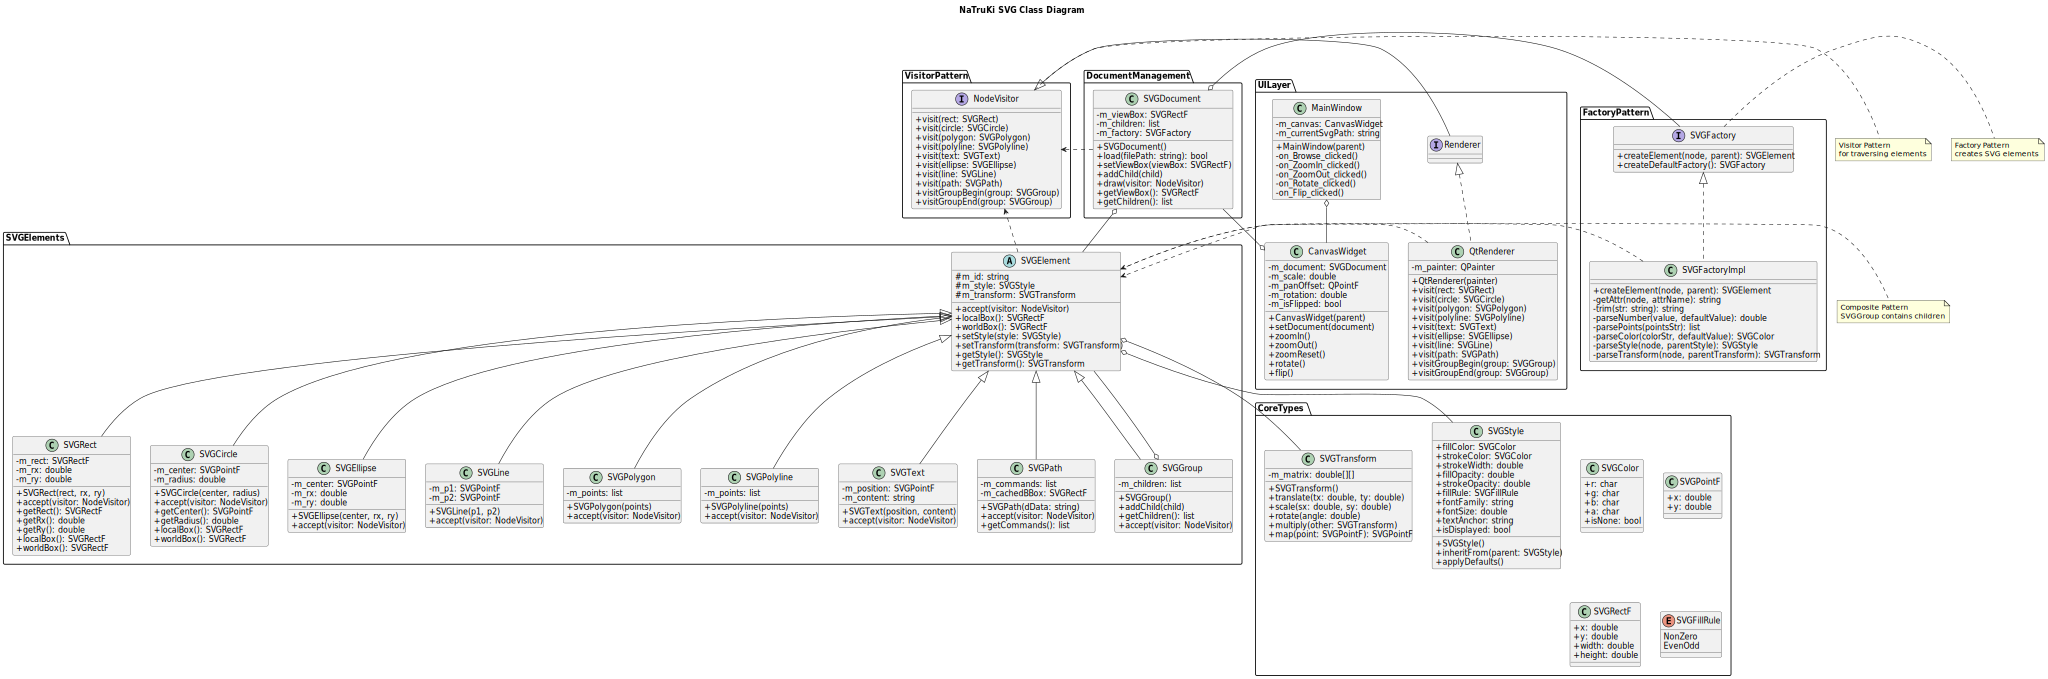
\includegraphics[width=\textwidth]{images/plantuml.pdf}
    \caption{Class Diagram của dự án NaTruKi}
    \label{fig:class_diagram}
\end{figure}

Để xem rõ hơn, nhóm cũng đã có để chi tiết \code{Class Diagram} ở trong \code{resources/plantuml.svg}.

\subsection{Xử lý SVGPath}

SVGPath là phần tử phức tạp nhất trong SVG vì nó có thể biểu diễn bất kỳ hình dạng nào thông qua chuỗi lệnh trong thuộc tính \texttt{d}. Một path có thể chứa các lệnh di chuyển (M/m), vẽ đường thẳng (L/l, H/h, V/v), đường cong Bezier (C/c, S/s, Q/q, T/t), và đóng đường (Z/z). Điểm đặc biệt là mỗi lệnh có hai dạng: chữ hoa (tọa độ tuyệt đối) và chữ thường (tọa độ tương đối), đồng thời một số lệnh có thể lặp lại nhiều tham số mà không cần ghi lại ký tự lệnh.

Để xử lý path, dự án sử dụng thuật toán phân tích cú pháp dựa trên máy trạng thái hữu hạn (Finite State Machine) \cite{wiki:fsm}. Thuật toán duyệt từng ký tự trong chuỗi \texttt{d}, phân biệt giữa lệnh và tham số số, sau đó chuyển đổi các tọa độ tương đối thành tuyệt đối để thuận tiện cho tính toán. Đối với rendering, các lệnh path được chuyển thành \texttt{QPainterPath} của Qt6, trong khi việc tính bounding box yêu cầu duyệt qua tất cả các điểm điều khiển và điểm cuối của mỗi lệnh. Một thách thức quan trọng là xử lý lệnh M đặc biệt: tọa độ đầu tiên sau M là moveTo, nhưng các tọa độ tiếp theo được hiểu ngầm định là lineTo.

\begin{table}[H]
\centering
\begin{tabular}{lll}
\textbf{Lệnh} & \textbf{Ý nghĩa} & \textbf{Xử lý} \\
\hline
M/m & Move to (di chuyển bút) & Đặt vị trí hiện tại, sau đó implicit L \\
L/l, H/h, V/v & Line to (vẽ đường thẳng) & Chuyển thành lineTo trong QPainterPath \\
C/c, S/s, Q/q, T/t & Bezier curves & Chuyển thành cubicTo hoặc quadTo \\
A/a & Elliptical arc & Tính toán cung ellipse phức tạp \\
Z/z & Close path & Nối điểm cuối về điểm bắt đầu subpath \\
\hline
\end{tabular}
\caption{Các lệnh SVG Path và cách xử lý}
\end{table}

\subsection{Xử lý SVGGroup - Pattern Composite}

SVGGroup đại diện cho thẻ \texttt{<g>} trong SVG \cite{mdn:svg} cho phép nhóm nhiều phần tử con lại với nhau và áp dụng style cũng như transform chung. Đây chính là thể hiện của Composite Pattern trong thiết kế, nơi SVGGroup vừa là SVGElement vừa chứa danh sách các SVGElement con. Khi một group có transform hoặc style, các thuộc tính này được kế thừa xuống tất cả các phần tử con theo cơ chế cascade tương tự CSS.

Thuật toán xử lý group dựa trên đệ quy và Visitor Pattern. Khi duyệt cây SVG, renderer gọi \texttt{visitGroupBegin} để lưu trạng thái hiện tại của QPainter (save), áp dụng transform của group, sau đó đệ quy duyệt tất cả các con, cuối cùng gọi \texttt{visitGroupEnd} để khôi phục trạng thái (restore). Điều này đảm bảo transform của group chỉ ảnh hưởng đến các con mà không làm thay đổi các phần tử khác. Đối với bounding box, thuật toán phải tính worldBox của tất cả các con (đã bao gồm transform của chúng), tìm hình chữ nhật bao quanh tất cả, rồi mới áp dụng transform của chính group đó lên kết quả.

\begin{table}[H]
\centering
\begin{tabular}{lll}
\textbf{Thao tác} & \textbf{Path} & \textbf{Group} \\
\hline
Parse dữ liệu & Phân tích chuỗi d phức tạp & Đơn giản, chỉ chứa children \\
Tính bounding box & Duyệt tất cả lệnh và điểm & Hợp nhất box của tất cả con \\
Rendering & Vẽ trực tiếp QPainterPath & Đệ quy render các con \\
Transform & Áp dụng lên toàn bộ path & Kế thừa xuống các con \\
\hline
\end{tabular}
\caption{So sánh xử lý SVGPath và SVGGroup}
\end{table}

\subsection{Mở rộng tính năng cho dự án có sẵn}

Việc thêm tính năng vào một dự án SVG viewer có sẵn đòi hỏi hiểu rõ kiến trúc hiện tại và áp dụng các design pattern phù hợp. Trong trường hợp dự án NaTruKi, kiến trúc ban đầu đã có sẵn xương sống cho các shape cơ bản (rect, circle, ellipse) với Visitor Pattern để rendering và Factory Pattern để parse XML. Khi cần thêm SVGPath và SVGGroup, nhóm phát triển không phá vỡ code cũ mà mở rộng theo nguyên tắc Open-Closed Principle.

Quy trình thêm tính năng bắt đầu bằng việc tạo class mới kế thừa từ SVGElement, implement các phương thức ảo thuần túy như \texttt{accept}, \texttt{localBox}, và \texttt{worldBox}. Tiếp theo, các phương thức \texttt{visit} mới được thêm vào interface NodeVisitor và implement trong QtRenderer. Factory cần được cập nhật để nhận diện và tạo phần tử mới từ XML node tương ứng. Điểm quan trọng là phải test kỹ lưỡng với các file SVG thực tế, đặc biệt chú ý đến các trường hợp edge case như path có lệnh lowercase, group lồng nhau nhiều tầng, hoặc transform phức tạp. Cách tiếp cận này đảm bảo code mới không ảnh hưởng đến chức năng cũ đã hoạt động ổn định.

\subsection{Feature Checklist}
Trong quá trình phát triển dự án, nhóm đã hoàn thành các tính năng sau đây trong milestone thứ hai:

\FloatBarrier
\begin{table}[H]
\centering
\caption{Feature Checklist - Milestone 2}
\label{tab:feature_checklist}
\begin{tabularx}{\textwidth}{|l|X|c|}
\hline
\textbf{STT} & \textbf{Tính năng} & \textbf{Trạng thái} \\
\hline
1 & Xử lý viewBox và preserveAspectRatio & \checkmark \\
\hline
2 & Xử lý các nhóm phần tử (Group) & \checkmark \\
\hline
3 & Xử lý các phần tử (path) & \checkmark \\
\hline
\end{tabularx}
\end{table}
\FloatBarrier

\section{Results}
Qua quá trình phát triển dự án, nhóm đã hoàn thành các tính năng sau đây trong milestone thứ hai. Dưới đây là kết quả render của 18 test cases khác nhau, thể hiện khả năng của ứng dụng trong việc xử lý các file SVG với độ phức tạp và cấu trúc khác nhau.

Xem thêm tại đây: \href{https://drive.google.com/drive/folders/1it5buU5MQ35VrvVOdTbFW3C-T1da-EMC?usp=sharing}{Google Drive}

\section{Conclusion}

Qua quá trình phát triển milestone thứ hai, nhóm đã thành công trong việc mở rộng ứng dụng NaTruKi SVG Viewer với hai tính năng quan trọng là SVGPath và SVGGroup. Việc bổ sung này không chỉ nâng cao khả năng hiển thị các file SVG phức tạp mà còn thể hiện được tính hiệu quả của kiến trúc phần mềm được xây dựng từ milestone đầu tiên. Nhờ áp dụng các design pattern như Visitor, Factory và Composite ngay từ ban đầu, quá trình thêm tính năng mới diễn ra thuận lợi mà không cần thay đổi code cũ, tuân thủ đúng nguyên tắc Open-Closed Principle.

SVGPath là phần tử phức tạp nhất được thêm vào, yêu cầu xử lý nhiều loại lệnh khác nhau với cả tọa độ tuyệt đối và tương đối. Thuật toán phân tích cú pháp dựa trên Finite State Machine đã được triển khai thành công để parse chuỗi path data, xử lý các trường hợp đặc biệt như implicit lineto sau moveto, và chuyển đổi sang QPainterPath để rendering. Đồng thời, SVGGroup với Composite Pattern cho phép nhóm các phần tử lại với nhau và áp dụng transform kế thừa, tạo nên cấu trúc cây phân cấp giống như DOM tree của SVG thực tế. Việc kết hợp giữa đệ quy và Visitor Pattern trong xử lý group đảm bảo transform được áp dụng đúng cách cho toàn bộ cây con.

Trong quá trình phát triển, nhóm đã học được nhiều bài học quý giá về thiết kế phần mềm mở rộng được. Việc planning kỹ càng về kiến trúc từ đầu giúp tiết kiệm rất nhiều thời gian khi cần thêm tính năng mới. Test với các file SVG thực tế từ nhiều nguồn khác nhau giúp phát hiện ra các edge case quan trọng như lowercase commands, nested groups, hoặc transform phức tạp. Ngoài ra, việc document code chi tiết và maintain git history rõ ràng cũng góp phần quan trọng vào sự thành công của dự án, đặc biệt khi làm việc nhóm với nhiều thành viên cùng đóng góp vào các phần khác nhau.